\documentclass[a4paper,spanish,12pt]{article}
\usepackage[spanish]{babel}
\usepackage[utf8]{inputenc}
\usepackage[pdftex]{graphicx}
\usepackage{vmargin}
\usepackage{float}
\usepackage{lastpage}
\usepackage{caratula}
\usepackage{url}
\usepackage{gensymb}
\usepackage{hyperref}

%\hypersetup{
%    colorlinks,
%    citecolor=black,
%    filecolor=black,
%    linkcolor=black,
%    urlcolor=black
%}

%%%%%%%%%%%%%%%%%%%%%%%%%%%%%%%%%%%%%%%%%%%%%%%%%%%%%%%%%%%%%%%%%%%%%%%%%%%%%%%%
% Para que las imagenes queden en donde esta el comando poner esto en el       %
% preambulo y usar los flags de posicion htp o htpb                            %
%%%%%%%%%%%%%%%%%%%%%%%%%%%%%%%%%%%%%%%%%%%%%%%%%%%%%%%%%%%%%%%%%%%%%%%%%%%%%%%%
%
% Alter some LaTeX defaults for better treatment of figures:
% See p.105 of "TeX Unbound" for suggested values.
% See pp. 199-200 of Lamport's "LaTeX" book for details.
%   General parameters, for ALL pages:
\renewcommand{\topfraction}{0.9}	% max fraction of floats at top
\renewcommand{\bottomfraction}{0.8}	% max fraction of floats at bottom
%   Parameters for TEXT pages (not float pages):
\setcounter{topnumber}{2}
\setcounter{bottomnumber}{2}
\setcounter{totalnumber}{4}     % 2 may work better
\setcounter{dbltopnumber}{2}    % for 2-column pages
\renewcommand{\dbltopfraction}{0.9}	% fit big float above 2-col. text
\renewcommand{\textfraction}{0.07}	% allow minimal text w. figs
%   Parameters for FLOAT pages (not text pages):
\renewcommand{\floatpagefraction}{0.7}	% require fuller float pages
% N.B.: floatpagefraction MUST be less than topfraction !!
\renewcommand{\dblfloatpagefraction}{0.7}	% require fuller float pages

%%%%%%%%%%%%%%%%%%%%%%%%%%%%%%%%%%%%%%%%%
% ECO Para jugar con el footer. 		%
\usepackage{fancyhdr}					%
%%%%%%%%%%%%%%%%%%%%%%%%%%%%%%%%%%%%%%%%%


%%\usepackage{hyphenat}
%%\exhyphenpenalty=10000
%%\hyphenpenalty=10000
\setmarginsrb{10mm}% left margin
{15mm}% top margin
{15mm}% right margin
{10mm}% bottom margin
{0mm}{20mm}{0mm}{30mm}% we needed -- related to headers and footers

%%%%%%%%%
\pagestyle{fancy}
\fancyhf{}

\fancyhead[LO, CE]{PedalerIA64 (Organización del Computador II)}
\fancyhead[RO, CE]{Laporte Matías}
\fancyfoot[C]{ \thepage\ de \pageref{LastPage} }


%%%%%%%%%%

\begin{document}


%*************************************************************%
%                                                             %
% CARATULA                                                    %
%                                                             %
%*************************************************************%
    \materia{Organizaci\'on del Computador II}

    \titulo{Trabajo Práctico Final: PedalerIA64}
    \subtitulo{\textit{Informe}}

    \integrante{Laporte Matías}{686/09}{matiaslaporte@gmail.com}
    
    \maketitle
    
%*************************************************************%
%                                                             %
% INFORME                                                     %
%                                                             %
%*************************************************************%

\section{Introducción}
\label{sec:introduccion}

\indent El presente Trabajo Práctico consiste en el desarrollo de diversos efectos de audio que se pueden encontrar en softwares de edición en el contexto musical (Cubase, Reaktor, Audacity, etc.), así como también en pedaleras (de allí el nombre del programa) para el caso específico de una guitarra.

\subsection{Proceso de desarrollo del TP}
\label{subsec:intro-desarrollo}
El proceso de desarrollo del \textbf{TP} consistió en realizar en primera instancia un rápido prototipado en Matlab/RStudio/Scilab (dependiendo de la disponibilidad de la computadora que se usara en ese momento; de ahora en más, me referiré a esos programas como \textbf{MRS}) de algoritmos y ecuaciones que se pudieran encontrar en Internet de diversos efectos. El uso de esos programas como primer acercamiento a un efecto facilitaba enormemente el trabajo, pues al utilizar un lenguaje de muy alto nivel se simplificaba el manejo de la lectura y escritura de los archivos, el espacio en memoria para los mismos, la manipulación de los datos (poder trabajar trabajar sobre un vector entero con una sola operación, por ejemplo), etc.\vspace{\baselineskip}

Una vez certificado que con ese algoritmo se consiguiera el efecto auditivo deseado, se pasó a desarrollarlo en \textbf{C}, siempre verificando que el resultado final de la señal coincidiera con el obtenido en \textbf{MRS}. Como utilizar el comando \textit{diff} de UNIX directamente sobre los archivos no siempre daba el resultado querido (aventuro a decir que por diferencias de aproximación entre \textbf{MRS} y \textbf{C}), se optó por otra metodología utilizando el programa \textbf{Audacity}, que se explicará en la sección \ref{subsec:chequeo-diferencias}.\vspace{\baselineskip}

Obtenido el resultado deseado utilizando \textbf{C}, se pasó finalmente a programar el mismo algoritmo en \textbf{Assembler}, haciendo uso de las instrucciones que ofrece el conjunto de instrucciones SSE para manejar múltiples datos con una única instrucción (SIMD). Se utilizaron instrucciones incluidas hasta la extensión SSE4 (principalmente por \textit{PTEST}, y \textit{ROUNDPS}/\textit{ROUNDSS}). Luego de obtener en \textbf{Assembler} un código que parecía aceptable (es decir, que no terminara abruptamente con un segfault), se comenzó con un proceso iterativo de corrección, mediante la comparación del archivo de audio obtenido con el de \textbf{C}, utilizando \textbf{Audacity} como se mencionó previamente. Las diferencias entre ambos muchas veces provenían de casos bordes, que se los mencionará en la sección \ref{subsec:problemas-en-desarrollo}.\vspace{\baselineskip}

El objeto de la programación en \textbf{C} además de Assembler, si bien implica el ''doble'' de trabajo, se debe a dos puntos en particular. En primer medida, era una buena manera de poder bajar el nivel del código original en \textbf{MRS}, despojándolo de las bondades que dichas herramientas ofrecen. Por otro lado, tener el código en \textbf{C} sirve también para comparar la mejora de rendimiento con el uso de las instrucciones SIMD. \vspace{\baselineskip}

Para calcular el rendimiento en ambos lenguajes se utilizó la librería \textit{Tiempo.h} utilizada por la cátedra en el \textbf{TP N\degree2} del 1er. Cuatrimestre de 2011. Cuando los resultados con la misma no eran satisfactorios (p.ej., \textbf{Assembler} era más lento que \textbf{C}), se procedió a utilizar una herramienta de profiling (\textbf{callgrind} en conjunto con \textbf{KCacheGrind}, se hablará de ellas más adelante) para poder identificar dónde exactamente estaban las secciones lentas del código en \textbf{Assembler}, y poder tomar medidas para resolverlo. De los casos puntuales donde se utilizó esto se hablará en las secciones \ref{desarrollo}, \ref{analisis} y \ref{resultado}.\vspace{\baselineskip}

Se desarrolló también una rudimentaria interfaz gráfica para tratar de evitar la utilización de la línea de comandos (en particular por la cantidad de argumentos que hay que manipular para los diversos efectos) y que la utilización del programa sea más amigable. Se hablará de ella en la sección \ref{subsec:GUI}.

\newpage
\subsection{Audio}
\label{subsec:audio}

\begin{figure}[H]
    \centering
    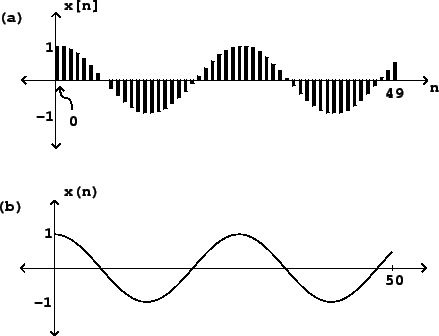
\includegraphics[scale=0.6]{imagenes/signals.png}
    \caption{Señales de audio}
    \label{fig:signals}
\end{figure}

Simplificándolo extremamente, una señal de audio (\textbf{(b)} en la imagen \ref{fig:signals}) es una representación del sonido, que puede ser visualizado como una curva continua (en el caso analógico, sus valores representan voltaje eléctrico) en función del tiempo. Al digitalizar una señal, se discretiza la curva (\textbf{(a)} en la imagen \ref{fig:signals}) tomando valores cada cierta cantidad de tiempo, lo que da lugar a la \textit{frecuencia de muestreo} (\textbf{sampling rate}, expresada como cantidad de muestras por segundo, unidad \textbf{Hz}). A la vez, cada uno de esos valores no puede ser expresado con precisión infinita, sino que al pasar al dominio digital, debe poder ser representado con una cantidad específica de bits, lo que origina la \textit{tasa de bits} (\textbf{bit rate}, \textit{resolución} de una señal de audio). \vspace{\baselineskip}

El formato de audio elegido para el \textbf{TP} es WAV, por ser uno de los más simples para manipular. Los datos correspondientes al audio no están comprimidos, por lo que es posible realizar directamente sobre ellos las operaciones necesarias para aplicar los diversos efectos. \vspace{\baselineskip}

La librería utilizada para el manejo de este archivo se verá en la sección \ref{subsec:libsndfile}.\vspace{\baselineskip}


\fbox{\begin{minipage}{42em}
Por recomendación del profesor durante la presentación del proyecto de \textbf{TP}, en el archivo de audio final obtenido luego de la aplicación de alguno de los efectos, la \textit{señal seca} (\textit{dry sound/dry signal}, sin efecto) va por un canal, y la \textit{señal húmeda} (\textit{wet sound/wet signal}) por el otro. De este modo, se puede apreciar con mayor claridad el efecto en cuestión. Esto implica que todos los archivos de salida tendrán dos canales (\textbf{stereo}), a pesar de que el archivo de entrada pudiera haber tenido un único canal. En el caso de archivos de entrada con dos canales, se realiza un promedio de ambos (aunque esto sólo es válido en archivos stereo que mandan el mismo audio por los canales), y sobre ese nuevo ``canal'' se aplica el efecto correspondiente.
\end{minipage}}

\newpage
\subsection{Herramientas externas utilizadas}
\label{subsec:herramientas}
Además de los ya mencionados \textbf{Matlab}, \textbf{RStudio}, y \textbf{Scilab}, se utilizaron las siguientas herramientas desarrolladas por terceros.

\subsubsection{libsndfile}
\label{subsec:libsndfile}
\textbf{libsndfile} es una librería de código abierto desarrollada en \textbf{C} para leer y escribir archivos de audio. Trabaja con el formato WAV, entre otros, por lo que se adaptaba a las necesidades del \textbf{TP}. La API puede consultarse aquí \footnote{\url{http://www.mega-nerd.com/libsndfile/api.html}}.\vspace{\baselineskip}

Una ventaja de la librería es que hace un pasaje de integer (tipo de datos utilizado en el formato WAV) a float, que es el tipo de datos utilizado para el \textbf{TP} \footnote{Originalmente se pensaba utilizar double, pero por recomendación del profesor se decidió pasar a float para poder procesar más datos}. Por otro lado, al leer un archivo utiliza una estructura propia llamada SF\_INFO, que incluye datos importantes del mismo (cantidad de canales, de muestras, entre otros), y que son necesarios en algunas porciones del \textbf{TP} por diversos motivos.

\subsubsection{Audacity}
\label{subsec:audacity}
\textbf{Audacity} es un editor multiplataforma de audio digital de código abierto y que en el \textbf{TP} se utilizó para realizar las comparaciones entre los archivos finales obtenidos de los diferentes efectos para cada lenguaje. De este modo, al no encontrar diferencias entre las señales de dos archivos diferentes, se podía corroborar que el algoritmo coincide con el efecto a aplicar.

\subsubsection*{Chequeo diferencias}
\label{subsec:chequeo-diferencias}
Para poder verificar si hay diferencias entre dos archivos de audio en Audacity, es necesario proceder del siguiente modo. Con el programa abierto, se arrastran los dos archivos hacia la ventana del mismo para que sean importados automáticamente (si es la primera vez, se va a preguntar si se quiere trabajar sobre los mismos archivos, o sobre una copia temporal de los mismos; por seguridad, se recomienda elegir esta última opción, y que el programa la recuerde).\vspace{\baselineskip}

Como ambos archivos son ``de salida'' (para nuestro programa), serán los dos stereo. Es necesario separar los canales de cada uno de los archivos, para compararlos entre sí. Hacer click sobre la flecha al lado del nombre del archivo, y clickear en ???? (o presionar la letra \textbf{n} del teclado). Separados ya los canales de ambos archivos, seleccionar el canal izquierdo del primer archivo (aparecerá con un color diferente al resto), e ir al menú de ``Efectos'', y elegir ``Invertir''. \vspace{\baselineskip}






\newpage

\section{Bibliografía tentativa}
\subsection{Libros}
\begin{thebibliography}{9}
 \bibitem{boulanger11}
  Richard Boulanger, Victor Lazzarini
  \emph{The Audio Programming Book},
  2011, The MIT Press, Massachussets (USA)
 
 \bibitem{moore90}
  F. Richard Moore,
  \emph{Elements of Computer Music},
  1990, Prentice Hall, New Jersey (USA)

  \bibitem{orfanidis10}
  Sophocles J. Orfanidis,
  \emph{Introduction to Signal Processing},
  \url{http://www.ece.rutgers.edu/~orfanidi/intro2sp/}
  
  \bibitem{roads96}
  Curtis Roads,
  \emph{The Computer Music Tutorial},
  1996, The MIT Press, Massachussets (USA)
  \bibitem{rocchesso03}
  Davide Rocchesso,
  \emph{Introduction to Sound Processing},
  \url{profs.sci.univr.it/~rocchess/SP/sp.pdf}
  
  \bibitem{smith99}
  Steven W. Smith,
  \emph{The Scientist and Engineer's Guide to Digital Signal Processing},
  Second Edition, 1999, California Technical Publishing, California (USA)
  
  \bibitem{zolzer11}
  Udo Zölzer,
  \emph{DAFX: Digital Audio Effects}
  Second Edition, 2011, Wiley and Sons, Hamburg (Germany)
\end{thebibliography}
  
\subsection{Internet}

\begin{itemize}
\item \url{http://www.mega-nerd.com/libsndfile/api.html}
\item \url{http://stackoverflow.com}
\item \url{https://ccrma.stanford.edu/~jos/}
\item \url{http://www.musicdsp.org/}
\item \url{http://www.kvraudio.org/}
\end{itemize}

\end{document}
